\documentclass[12pt,a4paper, openany]{book}

% Pacchetti utili
\usepackage[utf8]{inputenc} % codifica UTF-8
\usepackage[T1]{fontenc}
\usepackage{lmodern}
\usepackage{graphicx}       % per inserire loghi/immagini
\usepackage{setspace}       % per spaziatura
\usepackage{geometry}       % margini
\usepackage[export]{adjustbox}
\geometry{top=3cm,bottom=3cm,left=3cm,right=3cm}

\begin{document}
	% Pagina di copertina
	\begin{titlepage}
		\centering
		% Logo in alto (opzionale)
		% \includegraphics[width=0.25\textwidth]{logo.png}\par\vspace{1cm}
		
		{\Large \textsc{Università degli Studi di Torino}}\\[0.5cm]
		{\large Dipartimento di Informatica}\\[3cm]
		
		% Titolo
		{\Huge \bfseries Sistemi Operativi}\\[0.5cm]
		%{\LARGE Struttura, Progettazione e Implementazione}\\[2cm]
		
		% Autore
		{\large Autore}\\
		{\Large Francesco Martino}\\[1.5cm]
		
		% Relatore
		{\large Docente del corso}\\
		{\Large dottr. Marco Aldinucci}\\[3cm]
		
		% Data
		{\large Anno Accademico 2025--2026}
		
		\vfill
		
	\end{titlepage}\
	
	\chapter{Introduzione sui sistemi operativi}
	\begin{small} Il riassunto che segue si basa sul contenuto del Capitolo 1: Introduzione del testo "Sistemi Operativi", aggiornato alla decima edizione, coprendo i concetti fondamentali introdotti fino alla discussione preliminare della gestione dei file e delle strutture dati del kernel, prima della trattazione dettagliata sui file system (che inizia nel Capitolo 13)
		.
		La decima edizione evidenzia un grande impegno nel mantenere i contenuti al passo con la rapida evoluzione tecnologica
		. Sono state ampliate le tematiche relative ai sistemi per dispositivi mobili e alla virtualizzazione, e sono stati approfonditi gli aspetti legati alle architetture multicore. Questo capitolo in particolare include una copertura aggiornata sui sistemi multicore, la trattazione dei sistemi NUMA e dei cluster Hadoop, aggiungendo nuove motivazioni per lo studio dei sistemi operativi
		.
		\section{Introduzione}
		\subsection{Che cosa fa un sistema operativo} Un sistema operativo (SO) è un insieme di programmi (software) che gestisce gli elementi fisici di un calcolatore (hardware), fornisce una piattaforma per i programmi applicativi e funge da intermediario tra l'utente e la struttura fisica del calcolatore
		. I concetti fondamentali restano chiari nonostante l'evoluzione vertiginosa dei calcolatori, presenti ormai in ogni ambito, dai sistemi integrati nelle automobili ai server e ai dispositivi mobili
		.
		
		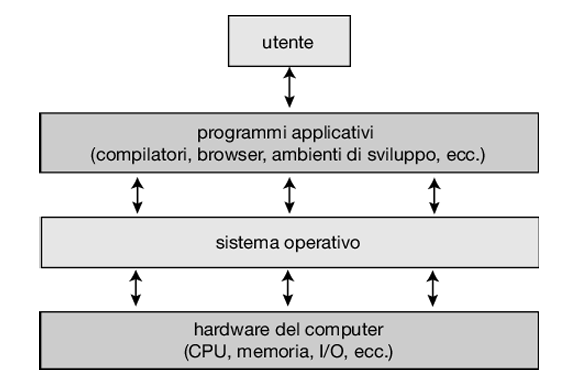
\includegraphics[width=10cm, center]{img/1.1.2.0}
		\subsection{Organizzazione di un sistema elaborativo} Il sistema elaborativo tipico comprende la CPU, la memoria, i dispositivi di I/O e i dispositivi di memorizzazione. La responsabilità cruciale del sistema operativo è allocare queste risorse ai programmi
		\newline
		
		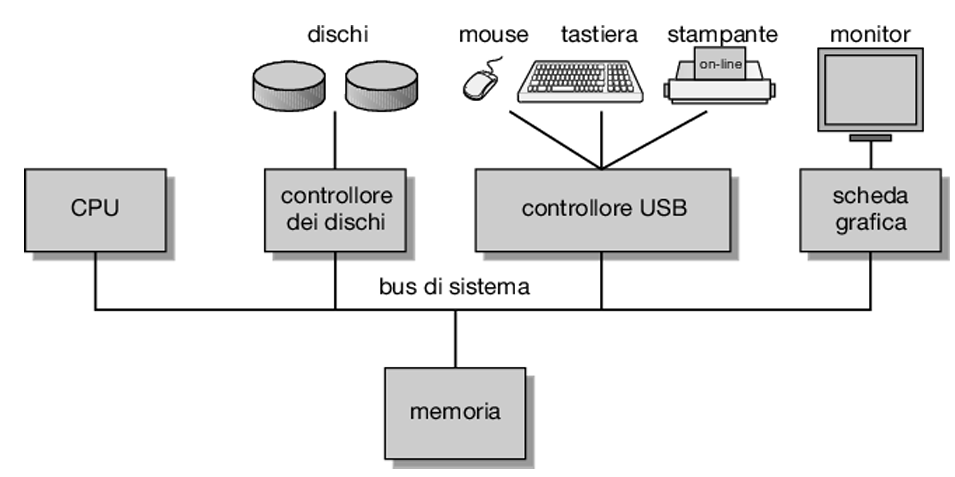
\includegraphics[width=10cm, center]{img/1.1.2.1}
		
		\subsubsection{Interruzioni} Le interruzioni (interrupt) sono un elemento cruciale nell'architettura di un calcolatore, utilizzate dai controller dei dispositivi per notificare il completamento di un'operazione di I/O
		. Quando si verifica un'interruzione, il controllo deve essere trasferito alla procedura di servizio appropriata. Sistemi operativi diversi, come Windows e Unix, utilizzano un vettore delle interruzioni — una tabella di puntatori memorizzata tipicamente agli indirizzi di memoria più bassi — per indirizzare rapidamente la procedura di gestione specifica
		.\newline
		• Processori Intel: Gli eventi da 0 a 31 (non mascherabili) segnalano condizioni di errore, mentre gli eventi da 32 a 255 (mascherabili) sono usati per le interruzioni generate dai dispositivi
		.\newline
		• Il meccanismo di interrupt implementa anche livelli di priorità, consentendo di posticipare le interruzioni a bassa priorità o di gestire immediatamente quelle ad alta priorità
		
		.
		
		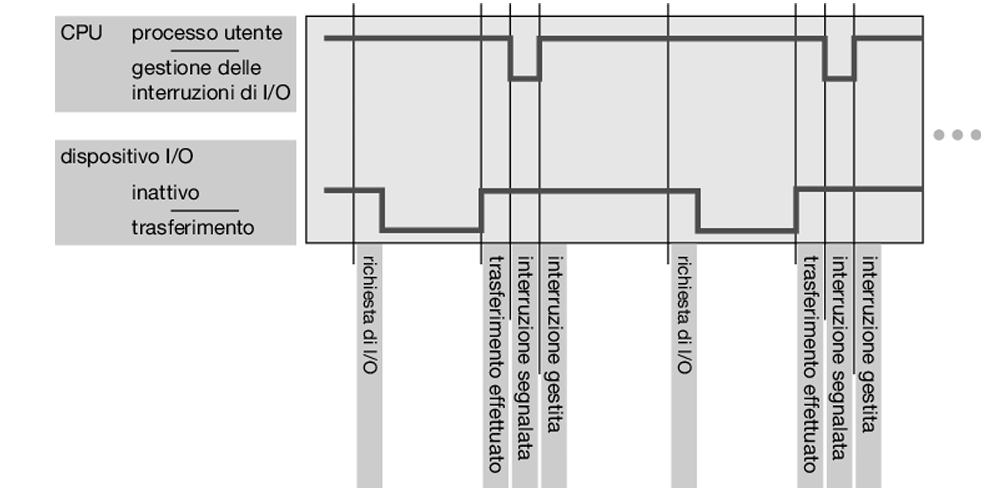
\includegraphics[width=10cm, center]{img/1.1.2.2}		
		
		\subsubsection{implementazione}
		 L’hardware della cpu dispone di un filo chiamato linea di richiesta di
		($interrupt-request line$) che la cpu controlla dopo l’esecuzione di ogni istruzione. Quando la cpu rileva che un controllore
		ha asserito un segnale sulla linea di richiesta di interruzione, legge il numero di interruzione e salta alla routine di gestione
		dell’interruzione utilizzando il numero letto come indice nel vettore delle interruzioni, per poi avviare l’esecuzione all’indirizzo
		associato a tale indice. Il gestore delle interruzioni salva le informazioni di stato che verranno modificate durante le operazioni,
		determina la causa dell’interruzione, esegue l’elaborazione necessaria, ripristina lo stato ed esegue un’istruzione di ritorno
		dall’interruzione ($return_from_interrupt$) per riportare la cpu allo stato di esecuzione precedente all’interrupt.
		
		
		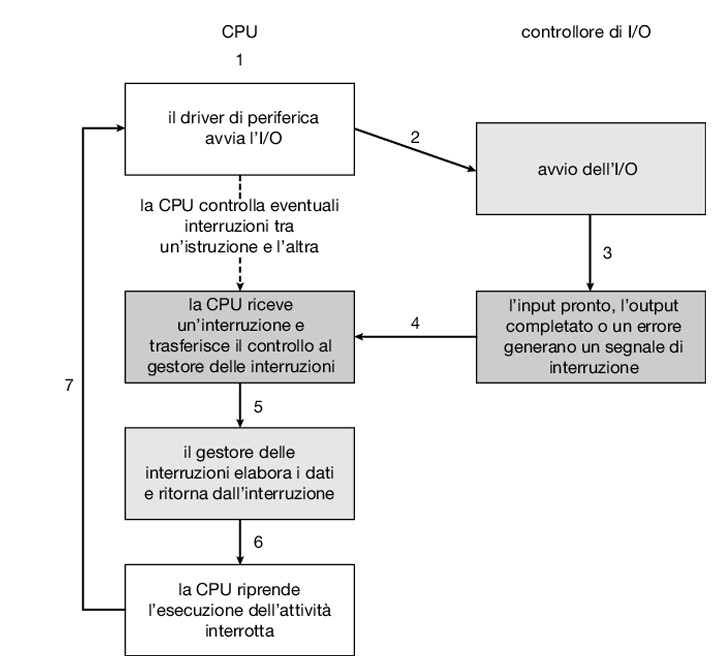
\includegraphics[width=10cm, center]{img/1.1.2.3}		
		
		 La maggior parte delle cpu ha due linee di richiesta di interruzione: una è non mascherabile (nonmaskable interrupt), riservata a
		eventi come errori irreversibili di memoria, mentre la seconda è mascherabile (maskable interrupt), ovvero può essere disattivata dalla
		cpu prima dell’esecuzione di sequenze di istruzioni critiche che non devono essere interrotte. L’interruzione mascherabile è quella
		utilizzata dai controllori dei dispositivi per richiedere un servizio		
		
		\subsubsection{Struttura della Memoria} La memoria centrale è un vasto vettore di byte, volatile, che perde il contenuto senza alimentazione elettrica
		. La CPU legge istruzioni e dati dalla memoria centrale (architettura di von Neumann)
		.\newline
		Per ovviare alla volatilità e alla capacità limitata della memoria centrale, la maggior parte dei sistemi include una memoria secondaria non volatile (nonvolatile storage, NVS) per conservare grandi quantità di informazioni, come dischi magnetici e dispositivi NVM (memoria non volatile elettrica, come la memoria flash e gli SSD)\newline
		. Tali dispositivi NVM sono trattati allo stesso livello delle unità a disco rigido in questa edizione.	 La memoria è organizzata in una scala gerarchica basata su velocità, costo, dimensione e volatilità, dove i livelli più vicini alla CPU (registri, cache) sono più piccoli e veloci.
		\newline
		All'avvio del computer, il primo programma che viene fatto partire è il programma di Bootstrap che si occupa di caricare il sistema operativo. Il bootstrap non può essere contenuto in RAM in quanto dispositivo di memoria volatile(perde i file allo spegnimento del circuito), viene quindi salvato all'interno di specifiche memorie chiamate "eeprom", programmabili elettricamente e cancellabili. 
		Come visto nel corso di Architettura degli elaboratori, tutte le informazioni vengono inserite nei registri/in memoria attraverso operazioni di load e store.
		
		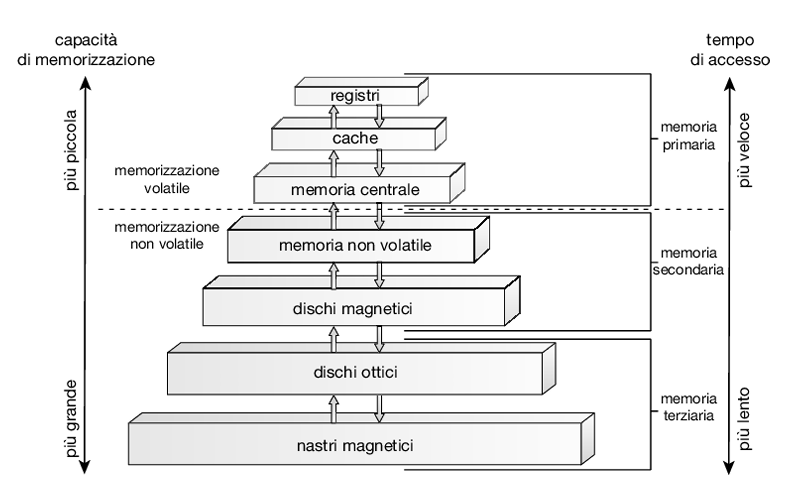
\includegraphics[width=10cm, center]{img/1.1.2.4}
		.
		\subsubsection{Gestione I/O}
		Includo solo una foto in quanto non c'è necessità di spiegare l'esistenza del DMA.\newline 
		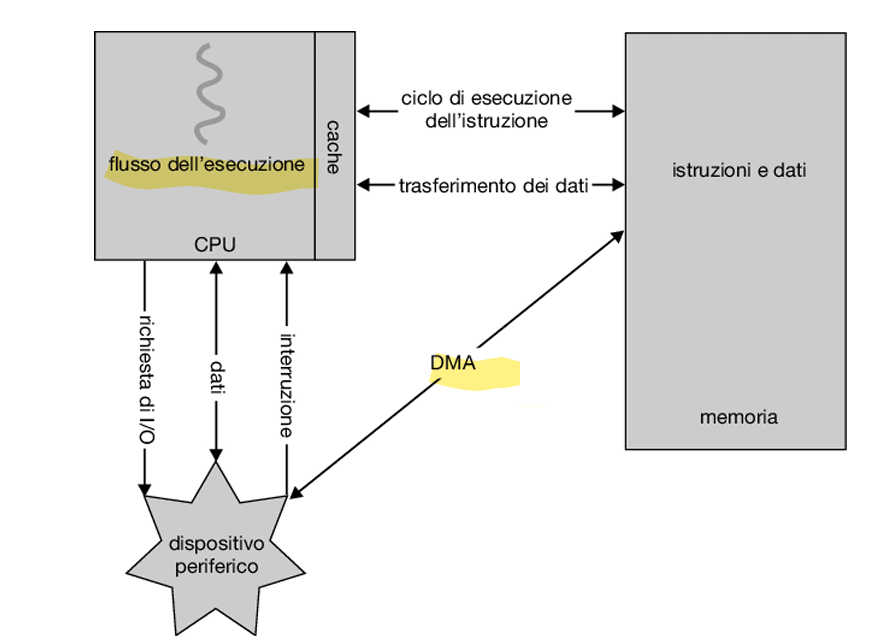
\includegraphics[width=10cm,center]{img/1.1.2.5}
		\subsection{Architettura degli elaboratori} I sistemi sono classificati in base al numero di unità di elaborazione
		.
		\subsubsection{Sistemi monoprocessore} Questi sistemi utilizzavano un solo processore con un unico nucleo di elaborazione (core)
		. Possono anche includere processori specializzati per compiti particolari, come i controller di dispositivi (disco, tastiera, video)
		.
		\subsubsection{Sistemi con accesso non uniforme alla memoria (NUMA)} Sebbene il titolo del paragrafo non sia esplicitamente riportato nelle fonti, il Capitolo 1 include una nuova trattazione sui sistemi NUMA
		. Un potenziale svantaggio di un sistema NUMA è l'aumento della latenza quando una CPU deve accedere alla memoria remota (non locale) attraverso l’interconnessione di sistema. I sistemi operativi tentano di minimizzare questo svantaggio attraverso un attento scheduling della CPU e una accurata gestione della memoria (come discusso nei Capitoli 5 e 10). I sistemi NUMA stanno diventando sempre più diffusi in ambienti server e di elaborazione ad alte prestazioni
		.
		\newpage
		\subsection{Attività del sistema operativo} I SO forniscono servizi essenziali agli utenti, tra cui
		:
		\newline
		• Interfaccia con l'utente (UI): Può essere a riga di comando 
		(CLI), grafica (GUI) o touch-screen
		.
		\newline
		• Esecuzione di un programma: Il SO deve caricare, eseguire e gestire la terminazione (normale o anomala) dei programmi
		.
		\newline
		• Operazioni di I/O: Il SO fornisce i mezzi per i programmi di eseguire I/O su file o dispositivi, garantendo protezione ed efficienza
		.
		\newline
		• Comunicazioni: Permette lo scambio di informazioni tra processi (nello stesso calcolatore tramite memoria condivisa o scambio di messaggi, o tra calcolatori in rete)
		.
		\newline
		• Rilevamento di errori: Il SO deve rilevare e correggere errori hardware (CPU, memoria, I/O) o software (errori nei programmi utente, come divisione per zero)
		.
		\newline
		\subsection{Gestione delle risorse} Il SO gestisce l'allocazione delle risorse hardware
		.
		\subsubsection{Gestione dei processi} Un processo è l'unità di lavoro attiva di un sistema, creata quando un programma passivo viene caricato in memoria
		. I moderni sistemi operativi sono spesso multiprogrammati, consentendo l'esecuzione concorrente di processi del sistema operativo e codice utente
		.
		La protezione dell'hardware è realizzata tramite la doppia modalità di funzionamento (modalità utente e modalità kernel/sistema)
		. L'esecuzione delle applicazioni utente avviene in modalità utente, ma le chiamate di sistema (interruzioni software) causano il passaggio automatico alla modalità kernel per accedere alle risorse privilegiate
		.
		\subsubsection{Gestione della memoria} La memoria centrale è l'unico grande dispositivo di memorizzazione a cui la CPU può accedere direttamente
		. Il SO ne gestisce l'allocazione, poiché affinché la CPU possa gestire dati da un disco o eseguire istruzioni, essi devono essere prima trasferiti in memoria centrale
		.
		\subsubsection{Gestione dei file} La gestione dei file è uno dei componenti più visibili di un sistema operativo
		. Il file è una raccolta di informazioni correlate definita dal suo creatore e registrata su memoria secondaria. La gestione dei file è trattata in dettaglio nei Capitoli 13, 14 e 15
		.
		\subsubsection{Gestione della memoria di massa} La maggior parte dei sistemi utilizza dischi magnetici e NVM come memoria secondaria principale
		. Il SO è responsabile delle attività connesse a questa gestione, tra cui montaggio/smontaggio delle unità, gestione dello spazio libero, allocazione dello spazio, scheduling del disco, partizionamento e protezione. L'efficienza complessiva del calcolatore dipende dalla velocità del sottosistema di gestione dei dischi e dagli algoritmi utilizzati. La memoria terziaria (come i nastri magnetici) ha uno scarso impatto sulle prestazioni ma richiede comunque gestione
		.
		\subsection{Sicurezza e protezione} Sebbene i meccanismi dettagliati siano trattati nei Capitoli 16 e 17, il SO è responsabile di garantire entrambi
		.
		\newline
		• Protezione (Protection): Limita l’accesso a risorse o oggetti da parte di processi o utenti, definendo controlli e vincoli
		.
		\newline
		• Sicurezza (Security): Consiste nel proteggere le informazioni memorizzate (dati e codice) e le risorse fisiche da accessi non autorizzati, alterazioni o distruzioni
		.
		\subsection{Virtualizzazione} La virtualizzazione è un settore fondamentale che influenza i sistemi operativi
		. La trattazione della virtualizzazione (inclusi i container applicativi) è stata ampliata in questa edizione. Le macchine virtuali (VM) consentono a sistemi operativi ospiti di essere eseguiti in un ambiente che appare loro come hardware nativo, garantendo protezione, gestione e limitazione delle risorse (Capitolo 18)
		.
		\subsection{Sistemi distribuiti} I sistemi distribuiti, trattati in dettaglio nel Capitolo 19
		, offrono vantaggi significativi. In tali sistemi, se più copie (repliche) dello stesso file sono mantenute su calcolatori diversi, è necessario garantire che ogni modifica su una replica si rifletta tempestivamente sulle altre per mantenere la coerenza
		.
		\subsection{Strutture dati del kernel} L'implementazione dei sistemi operativi si basa su strutture dati fondamentali utilizzate diffusamente dal kernel
		.
		\subsubsection{Liste Concatenate} Possono essere semplicemente concatenate
		, doppiamente concatenate (con riferimenti a successore e predecessore), o circolari. Offrono facile inserimento e rimozione, ma il tempo di accesso a un elemento è lineare O(n). Le liste sono usate spesso per costruire strutture più potenti, come pile (stack) e code
		.
		\subsubsection{Alberi} Gli alberi, come gli alberi di ricerca binari (che garantiscono prestazioni O(log n) nel caso peggiore se bilanciati), sono usati per rappresentare i dati in modo gerarchico
		. Ad esempio, Linux utilizza un albero binario di ricerca bilanciato (alberi Red-Black) nel suo algoritmo di scheduling della CPU
		.
		\subsubsection{Bitmap} Una mappa di bit (o vettore di bit) è un array di bit che rappresenta la disponibilità di un gran numero di risorse
		. Sono efficienti in termini di spazio e sono spesso usate per indicare la disponibilità dei blocchi sui dischi
		.
		\subsection{Ambienti d’elaborazione} L'elaborazione tradizionale (come l'ambiente d'ufficio con PC connessi in rete e server per file e stampa) è in continua evoluzione, con i confini tra i sistemi che si fanno più sfumati
		. Il capitolo introduce anche i sistemi real-time (elaborazione con vincoli di tempo precisi)
		.
		\subsection{Sistemi operativi liberi e open-source} Vengono menzionati sistemi come Linux (inclusa la distribuzione Ubuntu) e le varianti di Unix BSD (Freebsd, Netbsd, Openbsd, Dragonflybsd), con il codice sorgente disponibile per l'esame
		
		. \end{small}
	
\end{document}
